\documentclass{article}

% Language setting
% Replace `english' with e.g. `spanish' to change the document language
\usepackage[english,russian]{babel}
\usepackage{amsmath}

%графика
\usepackage{wrapfig}
\usepackage{graphicx}
\usepackage{pgfplots}


%%% Работа с картинками
\usepackage{graphicx}  % Для вставки рисунков
\graphicspath{{images/}{images2/}}  % папки с картинками
\setlength\fboxsep{3pt} % Отступ рамки \fbox{} от рисунка
\setlength\fboxrule{1pt} % Толщина линий рамки \fbox{}
\usepackage{wrapfig} % Обтекание рисунков и таблиц текстом

 % для диаграмм
\usepackage{pgf}
\usepackage{tikz}
\usepackage[utf8]{inputenc}
\usetikzlibrary{arrows,automata}
\usetikzlibrary{positioning}
\tikzset{
    state/.style = {draw, rounded corners, 
                 minimum width=22mm, minimum height=5mm, align=center},
}


\usepackage{tcolorbox}

% Set page size and margins
% Replace `letterpaper' with `a4paper' for UK/EU standard size
\usepackage[letterpaper,top=2cm,bottom=2cm,left=3cm,right=3cm,marginparwidth=1.75cm]{geometry}

% Useful packages
\usepackage{amsmath}
\usepackage{amssymb}
\usepackage{graphicx}
\usepackage{fixltx2e}
\usepackage[colorlinks=true, allcolors=blue]{hyperref}
\usepackage{pgf}
\usepackage{array}
\newenvironment{conditions}
  {\par\vspace{\abovedisplayskip}\noindent\begin{tabular}{>{$}l<{$} @{${}={}$} l}}
  {\end{tabular}\par\vspace{\belowdisplayskip}}

\usepackage{geometry}
\geometry{left=25mm,right=25mm,
 top=25mm,bottom=25mm}

\title{Quantitative Analytics.\\
Lectures. Week 1. \\
MARKET ORGANIZATION AND STRUCTURE. Организация рынка и его структура.}
\author{Григорий Агафонов}

% Колонтитулы
\usepackage{fancyhdr}
\pagestyle{fancy}
\renewcommand{\headrulewidth}{0.1mm}  
\renewcommand{\footrulewidth}{0.1mm}
\lfoot{}
\rfoot{\thepage}
\cfoot{}
\rhead{CMF-2022}
\chead{}

\begin{document}
\maketitle

% Оглавление
\setcounter{tocdepth}{1} % {2} - в оглавлении участвуют chapter, section и subsection. {1} - только chapter и section
\renewcommand\contentsname{Contents}
\tableofcontents
\newpage



\renewcommand{\labelitemi}{\tiny$\bullet$}
\renewcommand{\figurename}{Fig.}

\section{Что такое финансовая система?}
	Финансовая система обычно определяется через свои функции. Какие основные функции у финансовой системы?
	\begin{enumerate}
		\item \textbf{Удовлетворение целей} людей, использующих финансовую систему
		\begin{itemize}
			\item Получение кредита
			\item Сбережение денег
			\item Привлечение акционерного капитала (основное отличие от кредита здесь в том, что получатель делит долю в своем предприятии с акционерами)
			\item Управление рисками 
			\item Обмен активами 
			\item Трейдинг (суть трейдинга в заработке на изменении цен активов)
		\end{itemize}
	\item \textbf{Определение справедливой процентной ставки} (такая ставка уравновешивает общую сумму сбережений и кредитов в системе).
	\item \textbf{Эффективное распределение капитала}, т.е использование капитала наиболее оптимальным образом (плохой пример здесь - некоторые проекты на Kickstarter, которые получают финансирование, но не достигают заявленных целей)
		
	\end{enumerate}
\section{Классификация различных рынков}
Финансовые рынки классифицируют по разному, вот некоторые примеры:
\begin{itemize}
	\item Primary markets (компания выпускает новые ценные бумаги и ищет инвесторов с помощью инвестиционного банка) vs Secondary markets (ценные бумаги торгуются на бирже без участия компании)
	\item Money markets (рынок коротких долговых бумаг до 3х месяцв) vs Capital markets (рынок долгосрочных ценных бумаг, в основном акций)
	\item Traditional markets (акции, облигаций...) vs Alternative markets (криптовалюта) 
\end{itemize}
\section{Классификация различных активов}
Классифицировать активы можно по-разному:
\begin{itemize}
	\item Financial (акции, облигации, контракты...) vs Physical (можно потрогать руками  - сырье, недвижиость...) assets 
	\item Debt (практически безрисковые) vs Equity (рискованные) securities
	\item Private (не обращаются на бирже) vs Public (обращаются на бирже) securities
	\item Immediate delivery vs Future delivery
\end{itemize}
\section{Типы активов}
\begin{itemize}
	\item Securities 
	\item Currencies  
	\item Contracts (фьючерсы, опционы и тд)
	\item Commodities (газ, нефть и тд)
	\item Real assets (недвижимость)
\end{itemize}
\section{Ценные бумаги}

\begin{tikzpicture}[->,>=stealth']
\node (init)  [state,text width=3cm, ] {Securities};
\node (deb)  [state,text width=3cm,  below left=of init]    {Debt securities (Облигации)};
\node (eq)  [state, text width=3cm,xshift=-3cm, below right=of init]    {Equity securities (акции)};
\node (pool) [state,text width=5cm,  right=of eq]     {Pooled investments \\ (набор большого количества инвестиций)};
\node (stockprop) [state,text width=5.1cm,xshift=-2cm,below=of eq] 
 {\begin{tabular}{l}
  \parbox{4.9cm}{\begin{itemize}
   \item Обычные акции
   \item Привилегрированные акции (держатель получает дивиденты в первую очередь, но он лишен права голоса)
   \item Варранты (право купить акции компании в будущем, при соблюдении определенныйх условий)
  \end{itemize}
  }
  \end{tabular}};
  
 \node (poolprop) [state,text width=6.3cm,below=of pool]
 {\begin{tabular}{l}
  \parbox{5.9cm}{\begin{itemize}
   \item Mutual Funds (Российский аналог - паевые фонды. Такой фонд инвестирует в какой-то портфель акций и выпускает паи - доли этого  портфеля)
   \item Exchange-Traded Funds (такой же паевый фонд, но паи которого обращаются на бирже)
   \item Asset-Backed securities (пример - ипотечные облигации. Ипотечная облигация банка платит часть ипотечных платежей заемщиков держателю облигации)
   \item Hedge-Funds (инвестор покупает долю в хедж-фонде, с которой затем получает выплаты)
  \end{itemize}
  }
  \end{tabular}};
  
  \node (debterm) [state,text width=5cm,xshift=2.9cm, below left=of stockprop] {\begin{tabular}{l}
  \textbf{Классификация по} \\ \textbf{длительности}\\
  \parbox{4cm}{\begin{itemize}
   \item Долгосрочные (от 5 лет)
   \item Среднесрочные (от 2 до 5 лет)
   \item Короткосрочные (до 2 лет)
  \end{itemize}
  }\\[4em]
  \textbf{Классификация по} \\ \textbf{эмитентам}\\
  \parbox{4cm}{\begin{itemize}
   \item Государственные
   \item Корпоративные
  \end{itemize}
  }
  \end{tabular}};
  
  \node (useful) [state,text width=8.1cm,xshift=-1.5cm, below=of poolprop] {\begin{tabular}{l}
  \textbf{Полезно знать}\\
  \parbox{8 cm}{\begin{itemize}
   \item Bonds - долгосрочные облигации
   \item Notes - среднесрочные облигации
   \item Commercial paper - краткосрочные облигации
   \item Bills - государственные облигаци
   \item Certificates of deposit - банковские облигации
   \item Repurchase agreement - обязательство продать актив, купленный ранее
   \item Convertible debt - облигация, которая может быть сконвертирована в акцию при определенных условиях
  \end{itemize}
  }
   \end{tabular}};


\draw[->] (init) to (deb);
\draw[->] (init) to (eq);
\draw[->] (init) to (pool);
\draw[->] (pool) to (poolprop);
\draw[->] (debterm) to (useful);
\draw[->] (eq) to (stockprop);
\draw[->] (deb) to (debterm);



%\path (deb) 	edge[bend right=20]  (debterm);
 \end{tikzpicture}

\section{Контракты}
Рассмотрим несколько популярных типов контрактов:
\begin{enumerate}
    \item Форвард - обязательство купить(продать) актив в будущем по заранее оговоренной цене в определенную дату
    \item Фьючерс - стандартизированный форвард, который обращается на бирже
    \item Своп - обмен платежами между двумя контрагентами (например обмен платежа по плавающей процентной ставке на платеж по фиксированной)
    \item Опцион - право купить(продать) актив по определенной заранее известной цене в определенную дату
    \item Страховой контракт - производит выплату, в случае если происходит некоторое событие (пример такого контракта - страховка от дефолта CDS) 
\end{enumerate}
\section{Роли финансовых посредников}

\begin{tikzpicture}[->,>=stealth']
\node (corp)  [state,text width=5cm, ] {Corporations};
\node (IB)  [state,text width=5cm,below=of corp ] {Investments Banks};
\node (IB1) [state,text width=1cm,xshift=2cm,node distance=0.1cm,below left=of IB ] {Debt capital market};
\node (IB2) [state,text width=1cm,xshift=-2cm,node distance=0.1cm,below right=of IB ] {Equity capital market};
\node (ex)  [state,text width=7cm,yshift=-1.5cm,below=of IB ] {Exchange};
\node (cust)  [state,text width=3cm,left=of ex ] {Custodians};
\node (ch)  [state,text width=3cm,right=of ex ] {Clearing House};
\node (br) [state,text width=5cm,below=of ex ] {Brokers};
\node (FI) [state,text width=3cm,below=of br ] {Financial Institutions};
\node (cr) [state,text width=3cm,left=of FI ] {Corporations};
\node (people) [state,text width=3cm,right=of FI ] {People};
\draw[->] (corp) to (IB);
\draw[->] (IB1) to (ex);
\draw[->] (IB2) to (ex);
\draw[->] (cr) to (br);
\draw[->] (FI) to (br);
\draw[->] (people) to (br);
\draw[->] (br) to (ex);
\path (br) 	edge[bend right=50]  (ex);
\path (br) 	edge[bend left=50]  (ex);
\path (cust) 	edge[bend right=15]  (ex);
\path (ex) 	edge[bend right=15]  (cust);
\path (ex) 	edge[bend left=15]  (ch);
\path (ch) 	edge[bend left=15]  (ex);
\end{tikzpicture}


\textbf{Участники финансового рынка}
\begin{itemize}
\item\textbf{Exchange}(Биржа) - место, где происходит обмен ценными бумагами
\item\textbf{Brokers} - имеют право осуществлять сделки на бирже. Являются необходимыми посредниками при торговле
\item\textbf{Block brokers} - брокеры, которые открывают позиции по большими объёмами ценных бумаг
\item\textbf{Investment Banks} - помогают компаниям размещать ценные бумаги на первичном рынке
\item\textbf{Alternative trading systems} - альтернативные площадки, на которых люди обмениваются ценными бумагами
\item\textbf{Dealers} - имеет запас ценных бумаг, которыми он торгует с участниками рынка. Зачастую может обладать запасом не очень ликвидных бумаг. 
\item\textbf{Broker-Dealers} - брокер, который торгует ценными бумагами
\item\textbf{Primary-Dealers}(Первичные диллеры) - диллеры, которые торгуют с центральными банками или с министерствами финансов. В США существует 30 первичных диллеров, как правило это отделения крупных банков. Когда казначейство США выпускает новые облигации, первый выпуск распродается среди первичных диллеров
\item\textbf{Securitizers} - организации, которые занимаются превращением одних видов активов в другие в виде ценных бумаг. Примером таких бумаг могут быть ипотечные ценные бумаги
\item\textbf{Depository institutions} - организация, которая принимает депозиты и платит по ним проценты
\item\textbf{Prime Brokers} - организации, которые оказывают услуги очень крупным инвесторам.
\item\textbf{Insurance companies} -страховые компании
\item\textbf{Arbitrageurs} - организации, которые зарабатывают на арбитраже
\item\textbf{Clearing House} - это расчетная организация, которая производит расчеты по всем сделкам по итогам дня внутри биржи
\item\textbf{Custodians}(Депозитарии) - организации, которые хранят записи о правах собственности на ценные бумаги

\end{itemize}
\section{Длинные и короткие позиции}
\begin{itemize}
     \item Длинная позиция - это просто покупка актива
     \item Короткая позиция - трейдер сначала занимает актив, затем продает его на бирже, а через некоторое время он выкупает актив обратно и возвращает его.
\end{itemize}
Простыми словами инвестор, открывший длинную позицию, зарабатывает на росте цены актива, а инвестор, открывший короткую позицию, зарабатывает на падении цены.
Короткие позиции помимо спекулятивного интереса используются также для хеджирования рисков.



\begin{table}[h]
\caption{\label{tab:canonsummary} Открытие короткой позиции с $P_0=10\$\\$ $P_1=7\$\\$ и комиссией 2\$}
\begin{center}
\begin{tabular}{|c|c|c|c|c|c|c|}
\hline
\multicolumn{2}{|c|}{} & \multicolumn{3}{|c|}{Клиент} & \multicolumn{2}{|c|}{Брокер} \\
\hline
t & Описание & \$ & Число акций & Долг & \$ & Число акций\\
\hline
0 & - & 100 & 0 & 0 & 100 & 5\\
\hline
1 & Занять 5 акций & 100 & 5 & 5 & 100 & 0\\
\hline
2 & Продать 5 акций по 10 \$ за штуку & 150 & 0 & 5 & 100 & 0\\
\hline
3 & Купить 5 акций по 7 \$ за штуку & 115 & 5 & 5 & 100 & 0\\
\hline
4 & Вернуть 5 акций брокеру & 115 & 0 & 0 & 100 & 5\\
\hline
5 & Заплатить комиссию & 113 & 0 & 0 & 102 & 5\\
\hline
\end{tabular}
\end{center}
\end{table} 

 
Для коротких позиций существует такое понятие как \textbf{payments-in-lieu}. Оно означает, что в short позиции нужно отдавать дивиденты, выплачиваемые акцией владельцу этой акции. Часто говорят, что открытие коротких позиций - это рискованное мероприятие. Рискованное оно по трем причинам:
\begin{itemize}
    \item Долгосрочные тренды говорят о том, что в среднем все акции растут
    \item Открытие короткой позиции небесплатно, если акция не упадет, трейдер окажется в минусе
    \item Наличие payments-in-lieu
\end{itemize}

\section{Торговля с плечом}

С помощью займа можно открывать не только короткие, но и длинные позиции. Это называется торговля с плечом

\textbf{Leverage ratio (плечо)} - это соотношение стоимости открытия позиции к стоимости капитала инвестора
 
 При торговле с плечом риски инвестора значительно усиливаются. При резком падении рынка или при торговле с уровнем плеча гораздо выше двух может сложиться такая ситуация, когда инвестор не только потеряет все свои средства, но и останется должен брокеру. Для того чтобы защитить себя от риска невозврата брокер устанавливает специальные коэффиценты маржи \textbf{maintenance margin} ниже которого нельзя опускаться. Если инвестор опускается до этого уровня, то происходит запрос от брокера (\textbf{margin call}) с требованием пополнить счёт, иначе позиция закрывается.
\begin{equation}\label{margin call}
    \text{Margin call price }=P_0\cdot\frac{1-\text{initial margin}}{1-\text{maintenance margin}}
\end{equation}
где $P_0$ - первоначальная цена актива, initial margin - величина обратная leverage ratio, а maintenance margin устанавливается брокером.
 \\
 
 \textbf{Задача 1:}
 В начальный момент времени инвестор покупает $S=100$ акций по цене $P_0=50$ за штуку, причем известно, что он торгует с плечом initial margin которого $40\%$. Найдите доходность инвестора от продажи этих акций в следующий момент времени, если каждая акция заплатила дивиденты $D=5$ и цена одной акций выросла до $P_1=60$. Коммисия от сделки брокеру  $C=10$, а также известно, что брокер берет коммисию $q=5\%$ от суммы займа.  
 
 \textbf{Решение:}
\begin{align*}
    &\text{equity}=S\cdot P_0\cdot\text{initial margin}=100\cdot 50\cdot 0.4=2000&
    \\
    &\text{borrowed}=S\cdot P_0-\text{equity}=5000-2000=3000&
    \\
    &\text{return}=S\cdot(P_1-P_0)+S\cdot D-C-q\cdot\text{borrowed}=1340&
    \\
    &\text{return rate}=\frac{\text{return}}{\text{equity}+C}=\frac{1340}{2010}=66.7\%&
\end{align*}

\textbf{Задача 2:}
Начальная цена акции $P_0=120$ initial margin=40\% maintenance margin=25\%. Найдите цену акции, при которой случится margin call

\textbf{Решение:}
Можно просто воспользоваться формулой (\ref{margin call}):
\begin{flalign*}
  P=120\cdot\frac{0.6}{0.75}=96
\end{flalign*}
 Но давайте поймем, откуда берется эта формула. При торговле с плечом, занимаемая у брокера сумма 'застрахована' ,т.е на нее не начисляются убытки. 
 \begin{equation*}
     \underbrace{\text{Equity}}_{\text{убытки начисляются сюда}} +\qquad\quad \underbrace{\text{Borrow}}_{\text{застраховано}}
 \end{equation*}
 где в нашем случае :
 \begin{conditions}
 \text{Equity}&  $P_0\cdot\text{initial margin}=120\cdot 0.4=48$ \\
 \text{Borrow}     &  $P_0-\text{Equity}=120-48=72$    
\end{conditions}
 Предположим, что акция растёт или падает, ее новая цена $P^{'}$ тогда equity часть счёта инвестора будет меняться:
 \begin{equation*}
     \text{Equity}^{'}=\text{Equity}+(P^{'}-P_0)
 \end{equation*}
 Именно из этих соображений вводится maintenance margin:
 \begin{equation*}
     \text{maintenance margin}=\frac{\text{Equity}^{'}}{P^{'}}
 \end{equation*}
 Понятно, что чем меньше maintenance margin, тем меньше собственных денег на счете у инвестора. Теперь распишем подробнее:
 \begin{equation*}
     P^{'}\cdot\text{maintenance margin}=P_0\cdot\text{initial margin}+(P^{'}-P_0)
 \end{equation*}
 Отсюда и получается соотношение (\ref{margin call})
 
 \textbf{Замечание} мы вывели формулу из расчета на 1 акцию, но понятно, что ничего не поменяются если акций будет много.
 
 \section{Сделки на бирже}
 Для того чтобы совершить сделку, нужно отправить заявку(\textbf{trade order}) своему брокеру. Когда вы запустите биржевой терминал, вы увидите так называемый биржевой стакан(\textbf{Order Book}). Это таблица всех скопившихся заявок на покупку или продажу.
 \begin{figure}[h]
    \centering
   

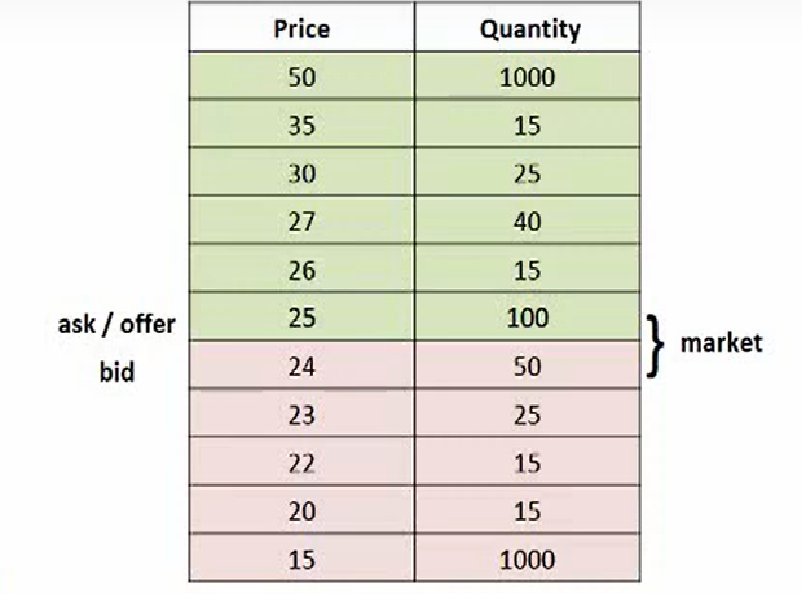
\includegraphics[width=4in,keepaspectratio]{bid ask.png}
\begin{center}
   \caption{\textbf{Биржевой стакан}} 
\end{center}
\end{figure}

 Красные ячейки на этом рисунке - это заявки на покупку(\textbf{bid}), зеленые - заявки на продажу(\textbf{ask)}. Совокупность наименьшей цены на продажу и наибольшей цены на покупку называется рынком (\textbf{market}). Разница между наименьшей ценой на продажу и наибольшей на покупку называется \textbf{bid-ask spread}.
 
 Bid-ask spread отражает ликвидность рынка, если ликвидность высокая, то Bid-ask spread небольшой и наоброт. Поэтому некоторые компании подписывают соглашения с \textbf{Market Maker'ами}, которые обязуются поддерживать узкие bid-ask spead'ы  в их акциях, таким образом, давая понять инвесторам, что эти акции ликвидны.
 
 В trade order помимо названия инструмента, цены, количества и параметра купить/продать содержится три группы инструкций:
 \begin{enumerate}
     \item \textbf{Execution} - как именно торговать
     \begin{itemize}
         \item Market orders  (выполняется полный объём по лучшим доступным ценам) vs limit orders (выставляется ограничение по цене, таким образом полный объем заявки может быть не реализован)
         \item All or nothing orders -заявка отменяется, если полный объем заявки не выполняется сразу (такую заявку можно сочетать например с limit order) 
         \item Hidden(iceberg) orders - такие заявки нужны, чтобы продать большое количество акций и не вызвать панику на рынке. Поступление акций в стакан происходит порциями, пока весь пакет акций не будет продан
     \end{itemize}
     \item \textbf{Validity} - когда заявка должна быть исполнена
     \begin{itemize}
         \item Good-till cancelled - заявка остается в системе, пока она не будет отменена
         \item Immediate or cancel - после того как часть заявки исполнена, оставшаяся часть снимается (например если есть заявка limit order immediate or cancel, то после того как часть заявки limit order исполняется, невыполненная часть не ждет исполнения, а отменяется)
         \item Good-on-close - заявка на покупку по цене закрытия
         \item Stop orders - смысл таких заявок в том, чтобы установить некоторое условие совершения сделки (пример продажа 100 акций по 20 если цена акции будет ниже 22)
     \end{itemize}
     \item \textbf{Clearing} - как именно расчитывать сделку. Когда поставлять активы (через день, два неделю...) и как будет производиться расчет по сделке.
     
 \end{enumerate}
 
 \section{IPO vs SPO}
 
 \begin{tikzpicture}[->,>=stealth']
 \node (n1)  [state,text width=3cm, ] {Capital markets};
 \node (ex)  [state,text width=3cm,xshift=-0.5cm, below right=of n1 ] {Secondary capital markets(биржи)};
\node (init)  [state,text width=3cm,below left=of n1 ] {Primary capital markets};
\node (IPO)  [state,text width=5cm,yshift=-0.5cm, node distance=0.5cm, below left=of init]    {Initial public offering (комания размещает свои ценные бумаги среди первоначального круга инвесторов с помощью инвестиционных банков)};
\node (SPO)  [state, text width=5cm,yshift=-0.5cm, node distance=0.5cm, below right=of init]    {Secondary public offering (компания выпускает дополнительные крупные пакеты акций и ищет новых инвесторов};
\node (prop) [state,text width=8.1cm,xshift=3cm, node distance=2.5cm, below left=of SPO] {\begin{tabular}{l}
  \textbf{Схемы взаимодействия с инвестиционным}\\ \textbf{банком}\\
  \parbox{8 cm}{\begin{itemize}
   \item Underwritten offering - инвестиционный банк заключает соглашение с компанией, что в случае, если он не найдет инвесторов на весь объем размещения акций, то сам банк выкупит оставшиеся акции. В таком случае банку выгодно занизить цены на акции, чтобы точно их продать
   \item Best efforts - банк не берет на себя обязательства по выкупу акций, в случае если он не найдет инвесторов. В таком случае есть вероятность, что на весь объем акций не найдется инвесторов 
  \end{itemize}
  }
   \end{tabular}};
   
\draw[->] (n1) to (init);
\draw[->] (n1) to (ex);
\draw[->] (init) to (IPO);
\draw[->] (init) to (SPO);
\draw[->] (IPO) to (prop);
\draw[->] (SPO) to (prop);
\end{tikzpicture}
 
 \section{Как работают современные биржи?}
 \begin{tikzpicture}[->,>=stealth']
 \node (n1)  [state,text width=3cm, ] {Типы рынков};
 \node (n2) [state,text width=7.1cm,xshift=-2cm, below right=of n1] {\begin{tabular}{l}
  \textbf{С точки зрения структуры}\\ \textbf{исполнения заявок}\\ 
  \parbox{7 cm}{\begin{itemize}
   \item Quote-driven markets(OTC) - на таких рынках первичным является котировка от диллера. В таком варианте рынков трейдеры взаимодействуют с диллерами
   \item Order-driven markets - биржевая торговля, в которой есть биржевой стакан. Первичными являются заявки инвесторов, которые соединяются между собой. Для этиъ рынков характерны наборы правил:
   \begin{itemize}
       
       \item Uniform pricing rule
       \item Discriminatory pricing rule
       \item Derivative pricing rule 
   \end{itemize}
   \item Brokered markets - на таких рынках, чтобы найти контрагента, люди используют брокеров. Пример - рынок недвижимости 
  \end{itemize}
  }
   \end{tabular}};
   
  \node (n3) [state,text width=6.1cm, below left=of n1] {\begin{tabular}{l}
  \textbf{С точки зрения организации}\\ \textbf{торговых сессий}\\
  \parbox{6 cm}{\begin{itemize}
   \item Call markets - акции торгуются в определенные моменты времени. Например выделяется полчаса на сбор заявок, по истечении этого времени устанавливается единственная цена по которой исполняется наибольшее количество заявок
   \item Сontinious markets - торговля ведется в любое время, пока рынок открыт. Так работает большинство бирж мира
  \end{itemize}
  }
   \end{tabular}};
   
   
   
   \draw[->] (n1) to (n2);
   \draw[->] (n1) to (n3);
 \end{tikzpicture}
 
 
\section{Типы эффективности финансовых систем}
Какая финансовая система будет эффективной? Такая которая, позволяет участникам рынка достигать своих целей.

Будем называть рынок полным(\textbf{complete market}) если 
\begin{itemize}
    \item Инвесторы могут сберегать по справедливой процентной ставке
    \item Заемщики могут выдвать кредиты со справедливой процентной ставкой
    \item Хеджеры могут управлять своими рисками
    \item Трейдеры могут получать нужные им активы
\end{itemize}
Если все эти функции выполняются при низких транзакционных издержках, то такая финансовая система обладает операционной эффективность(\textbf{operational efficiency})

Финансовая система обладает информационной эффективностью(\textbf{informational efficiency}) если цены на финансовые активы отражают всю доступную информацию

Финансовая система обладает эффективностью размещения(\textbf{allocation efficiency}) если капитал размещен наиболее эффективным образом
\newline
\section{Зачем регулировать финансовые рынки?}
\textbf{Проблемы}
\begin{itemize}
    \item Фрод и воровство
    \item Инсайдерская торговля
    \item Издержки на получение информации
    \item Дефолты
\end{itemize}
 
 \textbf{Цели, стоящие перед регуляторными органами}
 \begin{itemize}
     \item Защита инвесторов от фрода и дефолтов
     \item Помощь инвесторам в правильных оценках финансовых показателей
     \item Препятствие инсайдерской троговли
      \item Установление минимального уровня достаточности капитала
 \end{itemize}
 \end{document}
 
  